\documentclass[12pt, a4paper]{article}

\usepackage[utf8]{inputenc}
\usepackage[russian]{babel}
\parindent 0pt
\parskip 8pt
\usepackage{amsmath}
\usepackage{amssymb}
\usepackage{array}
\usepackage[left=2.3cm, right=2.3cm, top=2.7cm, bottom=2.7cm, bindingoffset=0cm]{geometry} % headheight=0pt,
\usepackage{hyperref}
\usepackage{graphicx}
\usepackage{multicol}
\usepackage{fancyhdr} 
\usepackage{extramarks}
\usepackage[usenames,dvipsnames]{color}
\usepackage{titlesec}
\usepackage{tikz}
\definecolor{grey}{RGB}{128,128,128}

\pagestyle{fancy}
\fancyhf{}
\lhead{Билет № 1.6}
\chead{Носители информации:\\ магнитные, оптические и на основе флеш-памяти, RAID}
\rhead{\thepage}
\lfoot{made with Ы}
\cfoot{}
\rfoot{\today}
\renewcommand\headrulewidth{0.4pt}
\renewcommand\footrulewidth{0.4pt}

\titlespacing*{\section}{0pt}{5pt}{0pt}
\titlespacing*{\subsection}{0pt}{5pt}{0pt}
\titlespacing*{\subsubsection}{0pt}{5pt}{0pt}

\begin{document}
\section{Дискета}
Магнитный диск, закрытый от залапывания пластиковым конвертом. В конверте есть прорезь, сквозь которую магнитная головка читает диск.\\
Две стороны диска разбиты на дорожки (цилиндры), дорожки разбиты на сектора. На одной дорожке 18 секторов.\\
Адресация: CHS (цилиндр - головка(поверхность) - сектор)\\
Объём сектора - 512байт, но это не чистые данные, а данные + хэш (CRC) + служебная информация(какая это дорожка и какой сектор, например) + ECC (коды исправления ошибок).
\begin{figure}[h]
    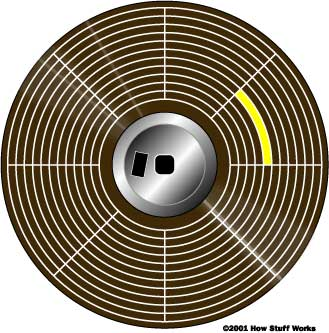
\includegraphics[scale=0.6]{./images/floppy-disk-track.jpg}
    \caption{Магнитный диск в дискете. Желтым выделен сектор}
    \label{fig:floppy-disk-track}
\end{figure}
\section{Про ECC и CRC}
\textbf{ECC} - коды исправления ошибок. В дисках используются коды Рида-Соломона. Такой код длины $M$ позволяет исправить $M / 2$ ошибок из всех $M + N$ битов. 
\section{Жесткий диск}

\section{}
\end{document}

